\section{Веб-приложение}\label{sec:-2}

\subsection{Аутентификация}\label{subsec:}
Стартовая страница.
На ней происходит аутентификация врача.
\begin{figure}[h]
    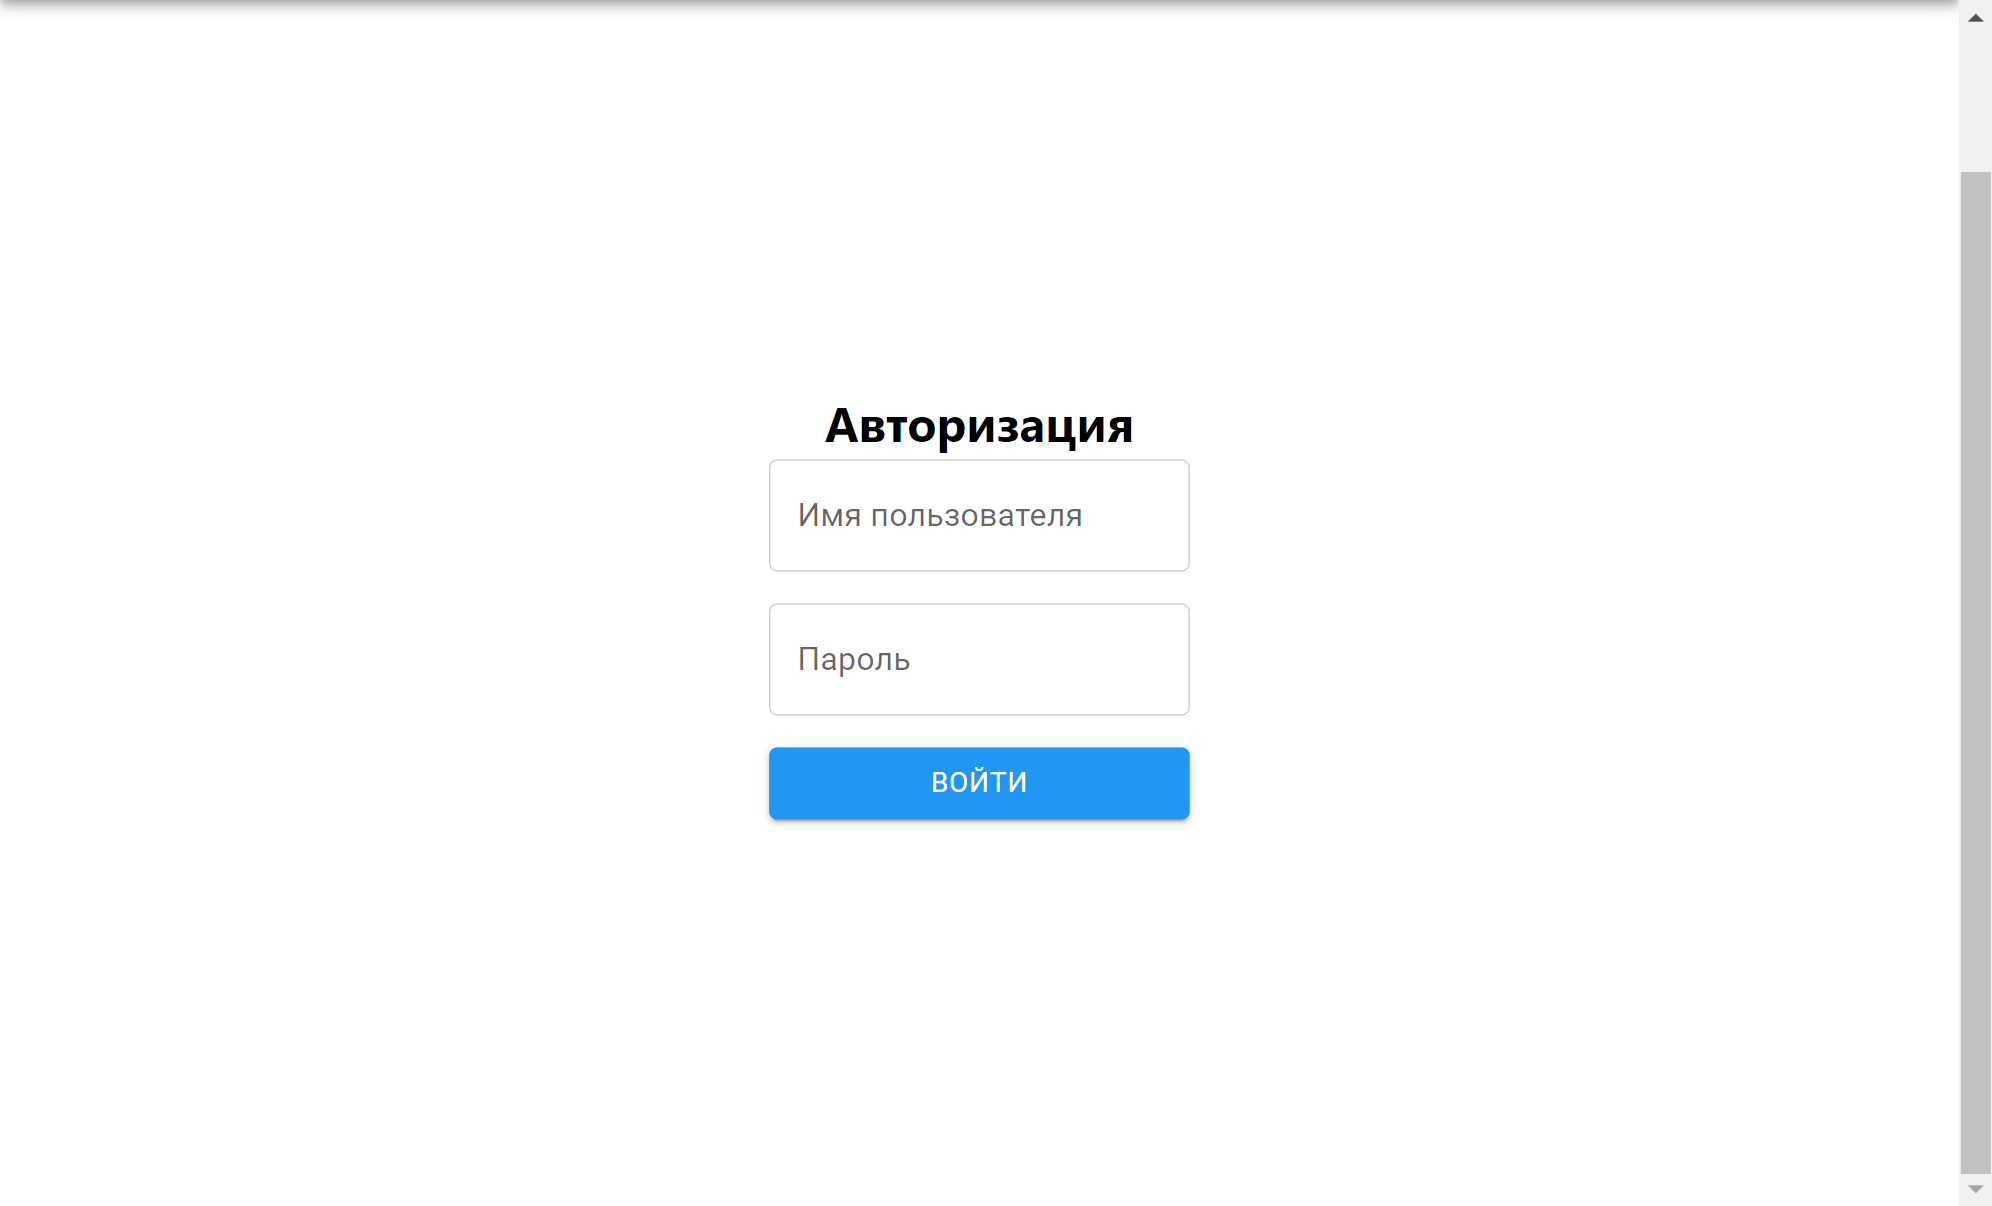
\includegraphics[scale=0.25]{images/screenshots/auth}
    \caption{Аутентификация.}\label{fig:figure4}
\end{figure}

\subsection{Главная страница}\label{subsec:-2}
На главной странице уже появляется хэдер, который есть во всем приложении, кроме страницы аутентификации.
В нем есть ссылки на саму главную страницу, на страницу регистрации пациента, так же имя врача, ссылка на его персональную страницу и возможность выхода из аккаунта.
В основном окне представлена таблица с результатами последних опросов, которые прошли пациенты.
В каждой строке нам важно знать, в какое время это произошло, с кем конкретно.
Важная графа с оценкой результатов опроса, она меняет свой цвет в зависимости от результата, чтобы врач мог сразу выделить отрицательные результаты и приступать к дальнейшим действиям.
\begin{figure}[ht]
    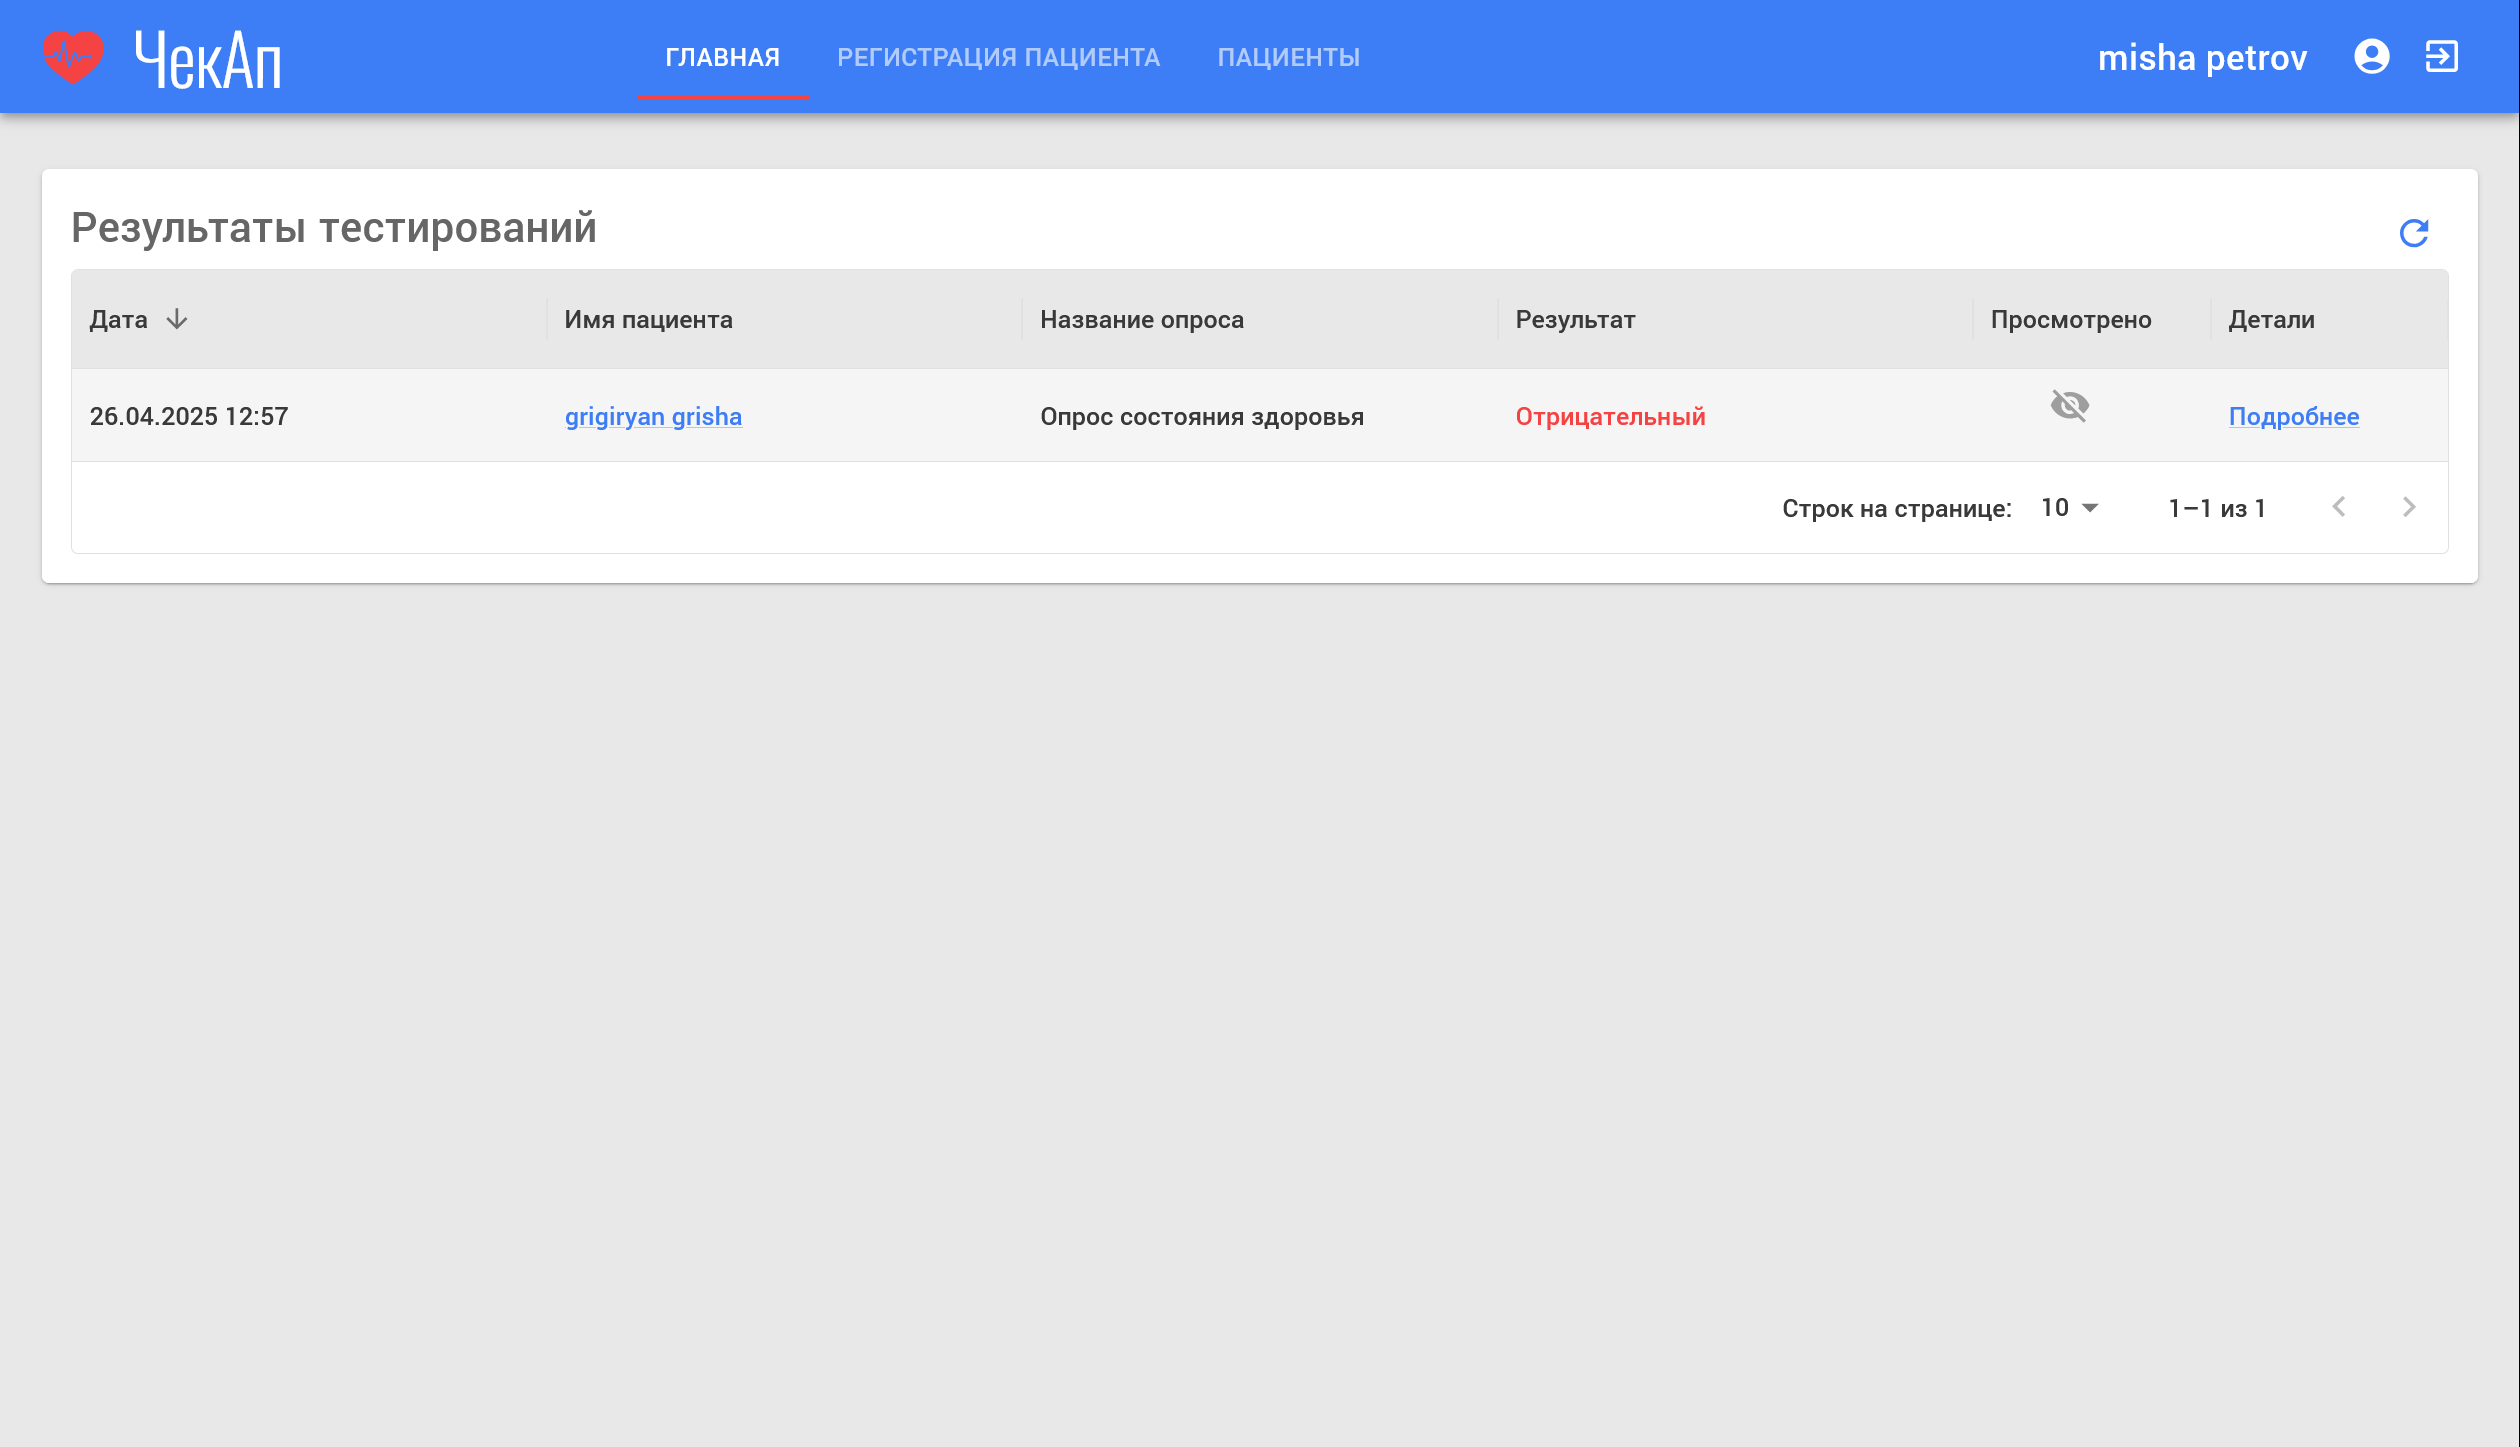
\includegraphics[scale=0.17]{images/screenshots/main_page}
    \caption{Главная страница.}\label{fig:figure5}
\end{figure}

\subsection{Опрос}\label{subsec:2}
На страницу с конкретным прошедшим опросом можно перейти по ссылке из главной страницы.
Здесь представлено подробно о пациенте и конкретные вопросы и ответы для более возможности оценки ответов лично врачом.
\begin{figure}[ht]
    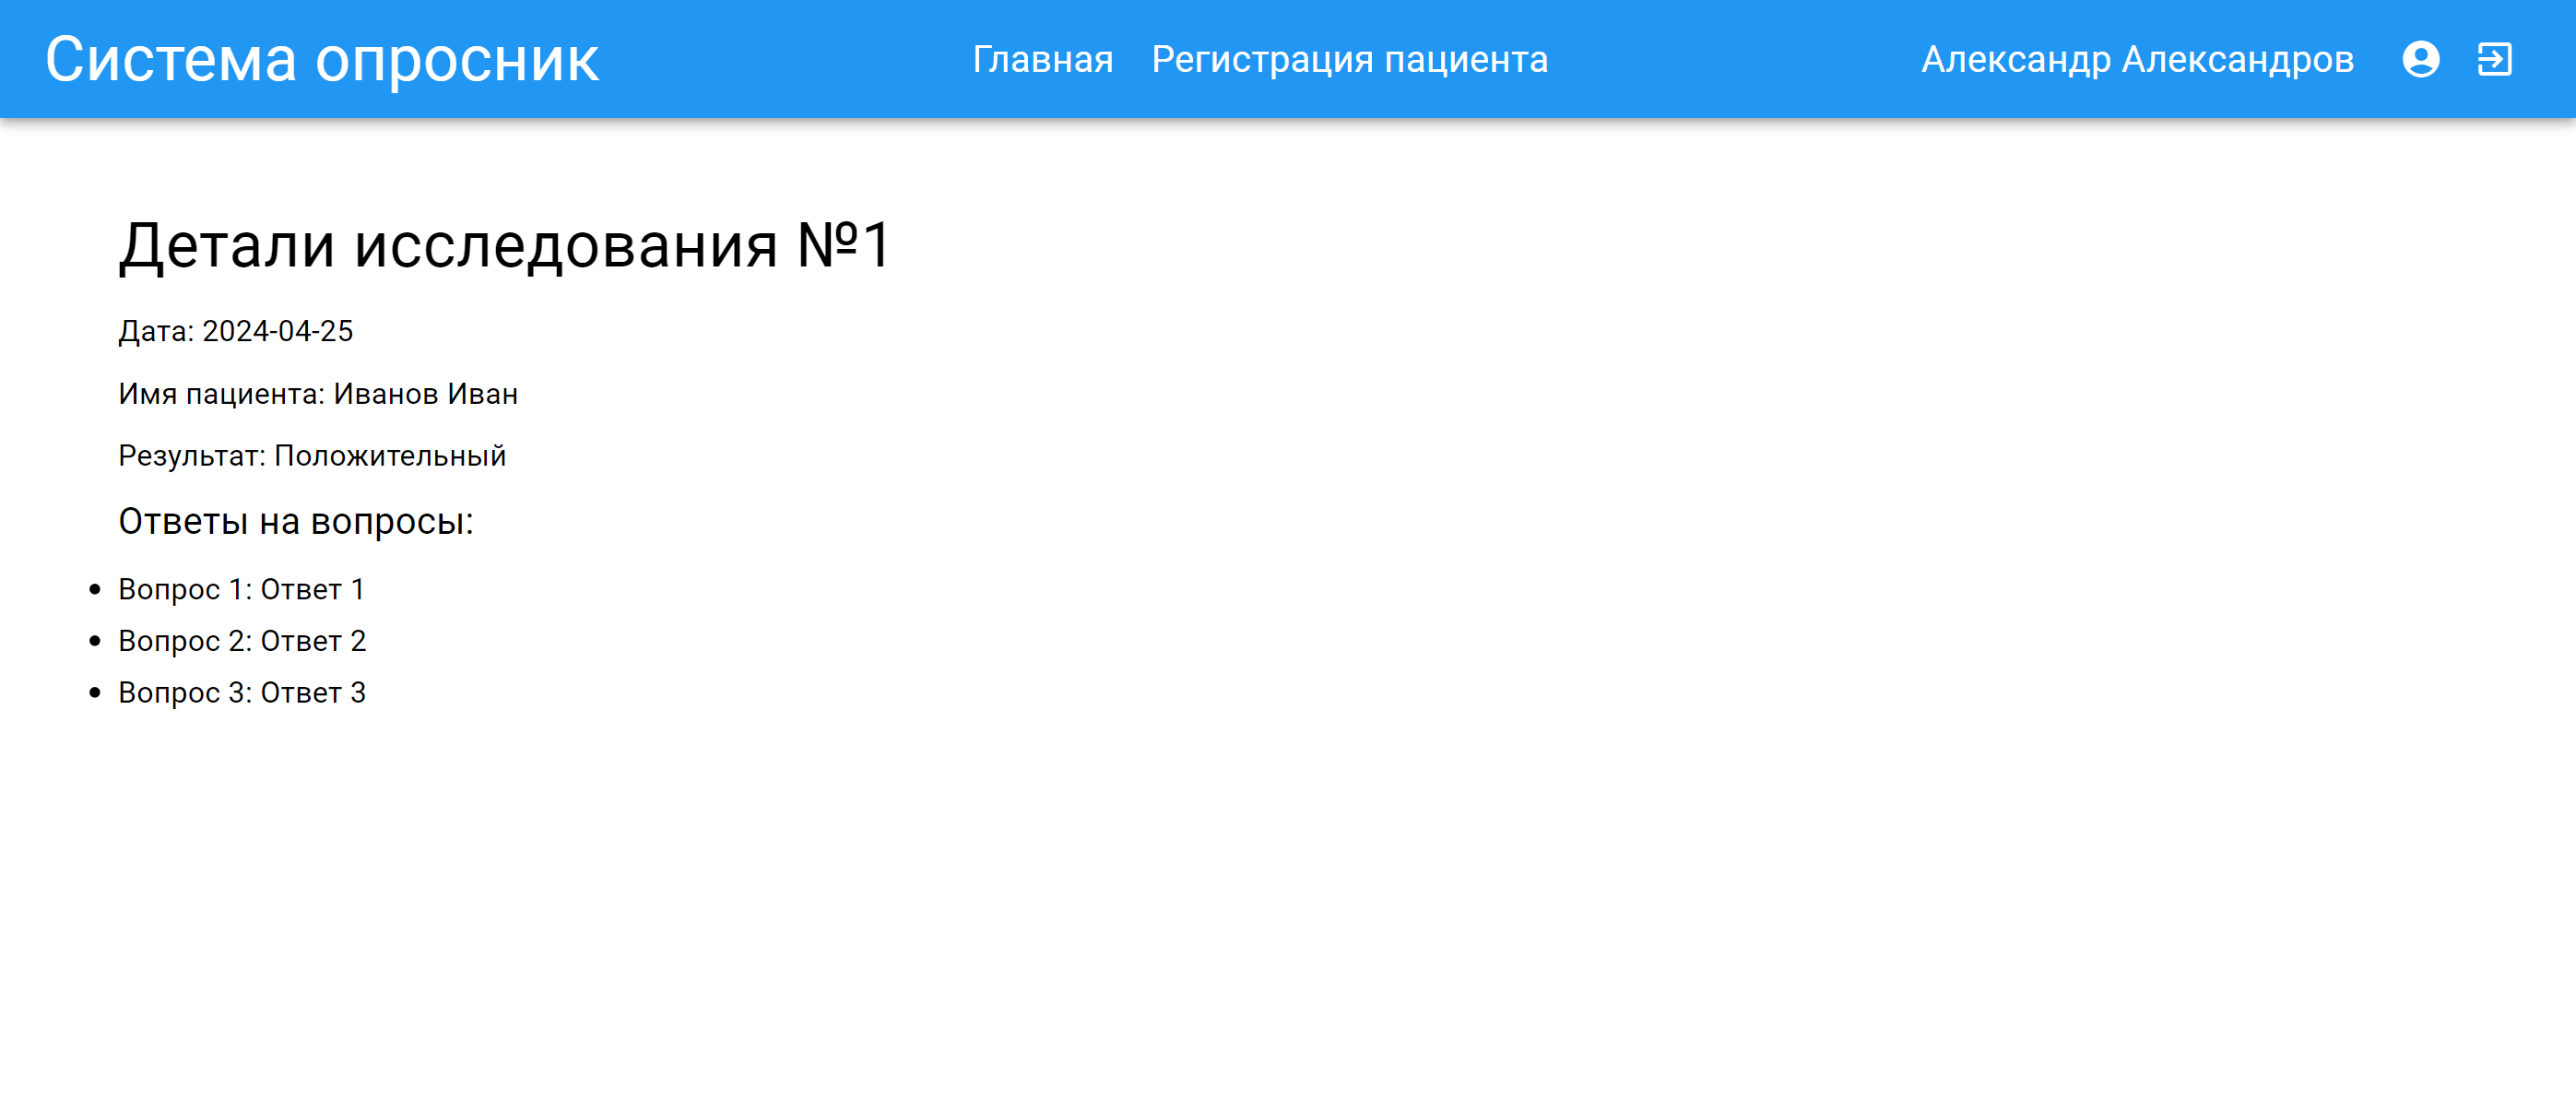
\includegraphics[scale=0.17]{images/screenshots/inquirer}
    \caption{Представление ответов в опросе.}\label{fig:figure6}
\end{figure}

\newpage
\subsection{Регистрация пациента}\label{subsec:-3}
На этой странице представлена форма для регистрации нового пациента (см.\ рис~\ref{fig:figure7})
\begin{figure}[ht]
    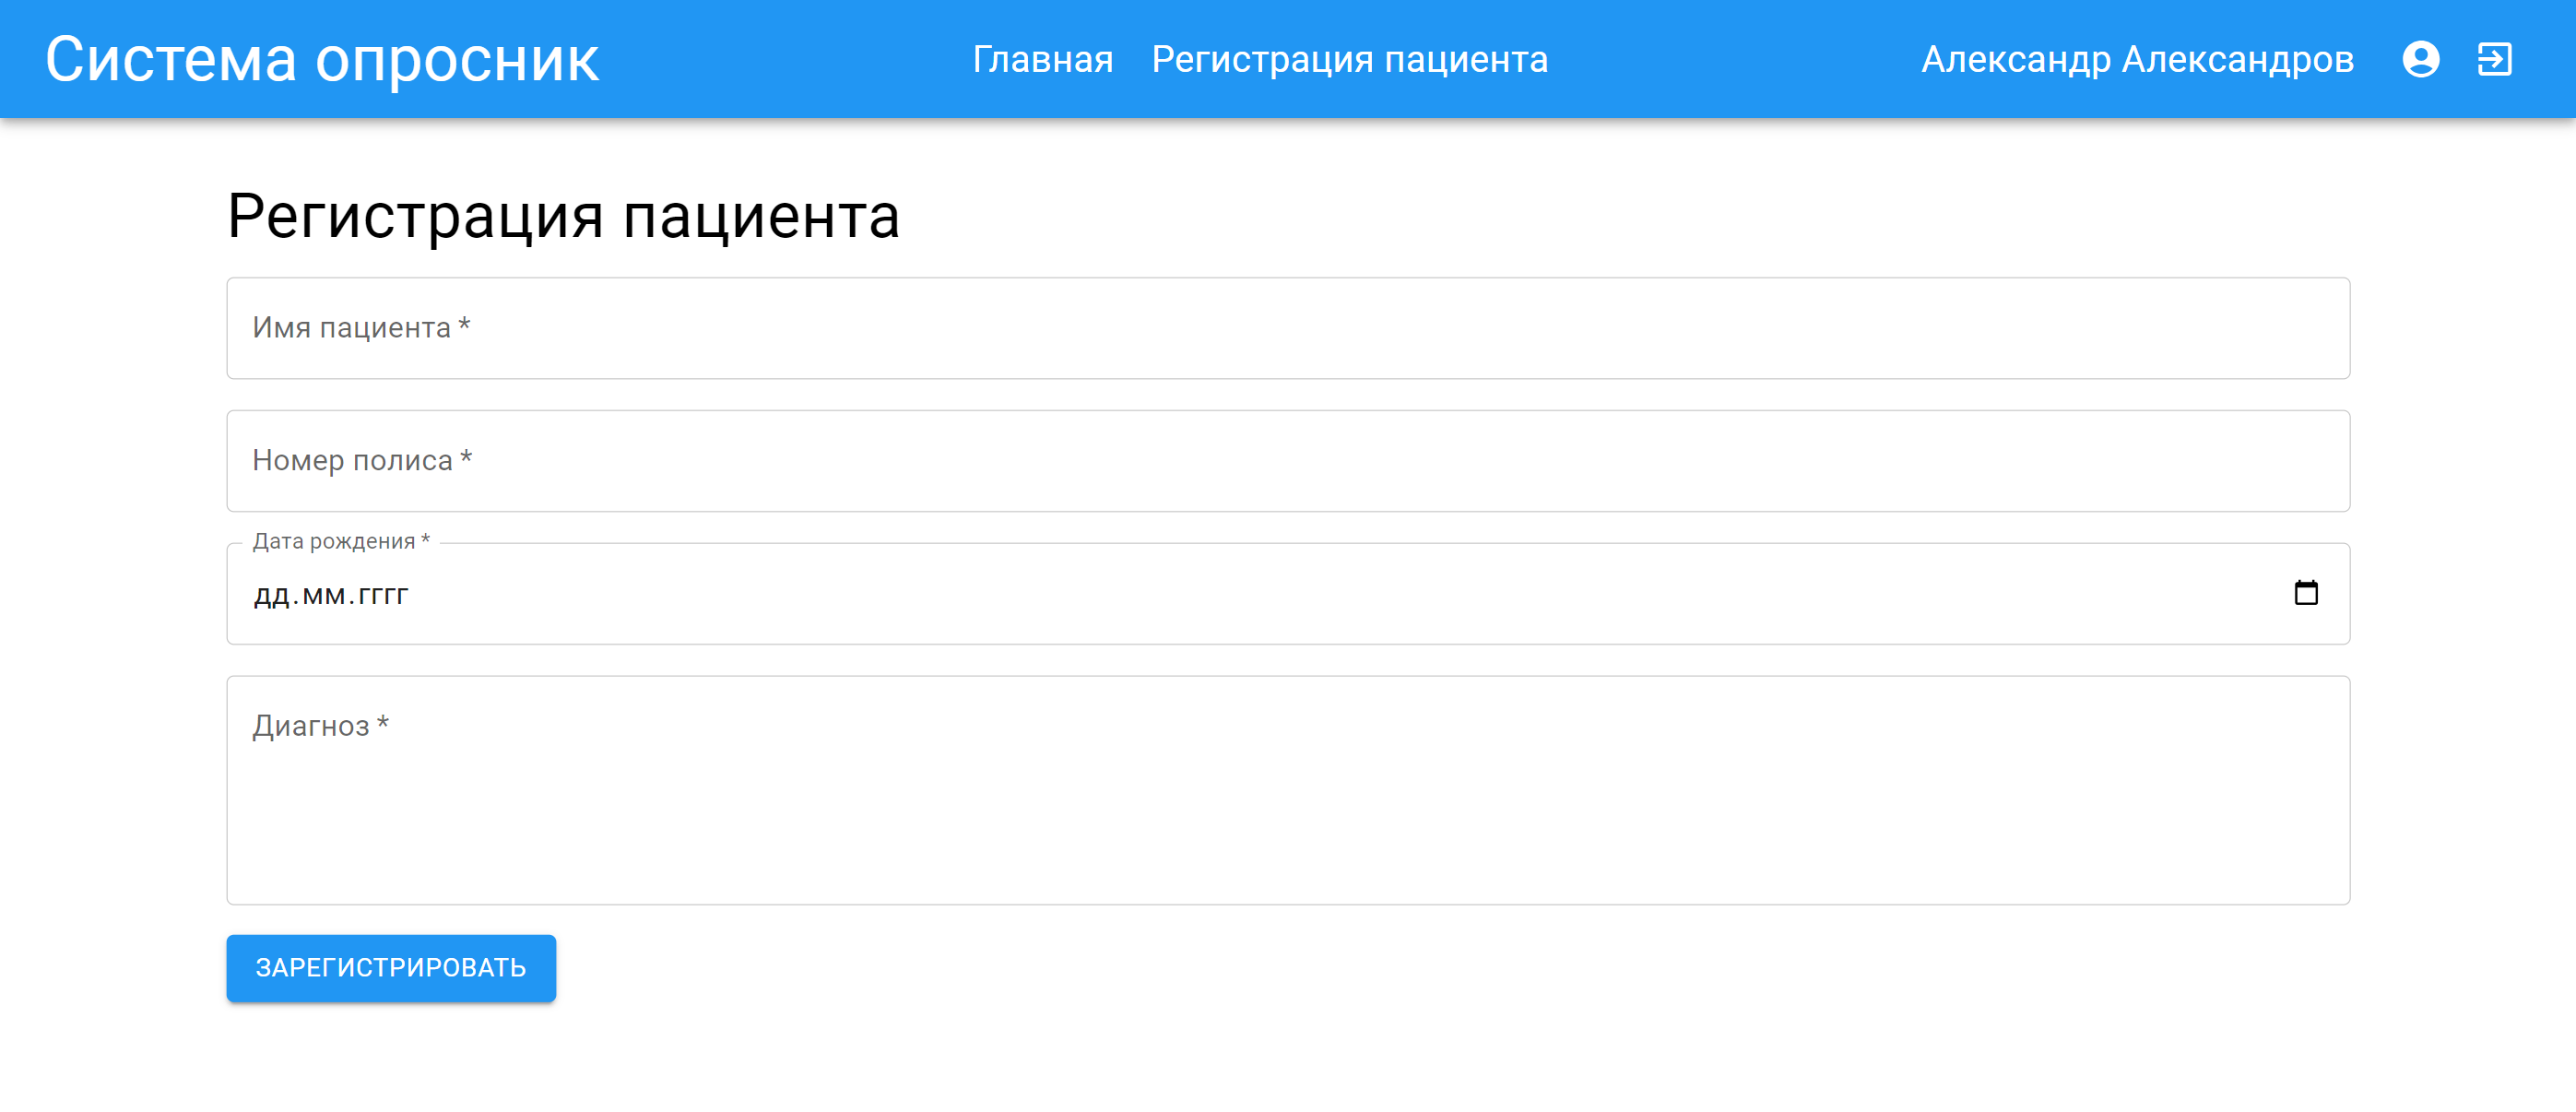
\includegraphics[scale=0.17]{images/screenshots/registration}
    \caption{Форма регистрации пациента.}\label{fig:figure7}
\end{figure}